%=====================================================================
\section*{Summary}
\note{4--5 sentences: the task, the method (identified state-space model, LQR with integral control and a Kalman filter (LQE), i.e.\ LQG),
the main rig result (zero mean steady-state error, both reference cases with one controller, push disturbance rejected, $|v|\le\SI{5}{V}$),
and the main limitation (unmodelled friction in the actuator gives a $\pm$1\,mm oscillation about the reference and 25--33\,\% overshoot going down).}

%=====================================================================
\section{Introduction}
% Short description of the system and the goal of the project.
\note{One paragraph on the task \cite{projdesc}: lift the payload to $x_0+\SI{15}{mm}$ and lower it to $x_0+\SI{5}{mm}$, with only $x$ measured.
List the specifications and say in two sentences how the report is organised.}

\begin{table}[H]\centering
\caption{Specifications (project description, Sec.~3.3) and where they are addressed.}
\begin{tabular}{lll}\toprule
Specification & Approach & Section\\\midrule
Full-state feedback, fast, little oscillation & LQR (Bryson weights) & \ref{sec:ctrl}\\
Unmeasured states estimated & Kalman filter (LQE) & \ref{sec:obs}\\
15$\to$5 and 20$\to$5\,mm, one controller & same gains, no retuning & \ref{sec:results}\\
Zero steady-state error & integral control & \ref{sec:ctrl}\\
Robust to model error, $\eta<1$, push & robustness checks over the parameter uncertainty, push test & \ref{sec:ctrl}, \ref{sec:sim}, \ref{sec:results}\\
$|v|\le\SI{5}{V}$, stroke 0--25\,mm & saturation + anti-windup, prefilter & \ref{sec:rt}\\\bottomrule
\end{tabular}\end{table}

%=====================================================================
\section{Mathematical Model}\label{sec:model}
% Equations for motor, ball screw, actuator mass, spring/damper and payload.
\note{Describe the rig (ball screw, BLDC motor, spring, payload, inductive sensor at the bottom). Explain each equation below in a sentence:
KVL, torque, ball-screw force with lead $l$ and $\eta$, Newton for the actuator and the payload. Why states relative to the equilibrium (operating) point (gravity drops out)
and why a linear model (LQR and Kalman need one, and the stroke is small).}

The screw ratio is $N = 2\pi/l$, so $\omega_m = N\dot y$. The motor and the ball screw give
\begin{align}
L\,\frac{di}{dt} &= v - R\,i - K_b\,\dot y, & K_b &= k_b N = \SI{22.6}{V/(m/s)},\\
M_e\,\ddot y &= K_f\, i - k_s (y-x) - b_s(\dot y-\dot x), & K_f &= \eta\, k_i N = \SI{22.6}{N/A},\\
m_l\,\ddot x &= k_s (y-x) + b_s(\dot y-\dot x), & M_e &= m_a + \eta J_m N^2,
\end{align}
where all positions are measured from the equilibrium (operating) point.

\subsection{State-Space Model}
% State vector, A, B, C matrices. Only x is measured.
With the state $\mathbf{x} = [\,i\;\; y\;\; \dot y\;\; x\;\; \dot x\,]^T$, input $v$ and output $x$:
\begin{equation}
A=\begin{bmatrix}
-R/L & 0 & -K_b/L & 0 & 0\\
0 & 0 & 1 & 0 & 0\\
K_f/M_e & -k_s/M_e & -b_s/M_e & k_s/M_e & b_s/M_e\\
0&0&0&0&1\\
0 & k_s/m_l & b_s/m_l & -k_s/m_l & -b_s/m_l\end{bmatrix},\quad
B=\begin{bmatrix}1/L\\0\\0\\0\\0\end{bmatrix},\quad
C=\begin{bmatrix}0&0&0&1&0\end{bmatrix}.
\end{equation}
The sensor is modelled as a first-order lag \cite{balluff}. This adds a sixth state $x_s$ with
$\dot x_s = (x-x_s)/\tau_s$, $\tau_s=\SI{10.6}{ms}$, and the output becomes $x_s$.

\note{Controllability and observability: the controllability and observability matrices have full rank, confirmed with the Hautus test (ctrb\_calc.m).
Give the open-loop poles (run plant\_model without outputs) and comment: the actuator behaves like an integrator, and the 2.5 Hz payload mode is lightly damped.}

%=====================================================================
\section{System Identification}\label{sec:ident}
% How ks and bs were found experimentally, and why this method was chosen.
\note{Why the time domain is the main method and the frequency domain a check (the project description allows both).}

\subsection{Spring Coefficient}
The spring coefficient $k_s$ was found with a static test. The spring
length was measured without load and with the payload hanging from it:

\begin{itemize}
  \item Unloaded length: 27 mm
  \item Loaded length: 65 mm
  \item Payload mass: $m_l = 0.51$ kg
\end{itemize}

The spring force equals the weight of the payload, so

\begin{equation}
  k_s = \frac{m_l g}{\Delta x} = \frac{0.51 \cdot 9.81}{0.065 - 0.027}
  \approx 131.7 \text{ N/m}
\end{equation}

This method was chosen because it is simple and only needs a length measurement.

\subsection{Damping Coefficient}
\note{Impulse response (payload released from a small perturbation, actuator held still), identified with the logarithmic decrement as in L2d and Tutorial 2 (identify\_bs.m).
One or two sentences on why: the payload mode is a second-order system $m_l\ddot x + b_s\dot x + k_s x = 0$, so its free decay gives $\zeta$ and $\omega_n$ directly.}
With the oscillation amplitudes $O_1$ and $O_{n+1}$ of two peaks $n$ cycles apart,
\begin{equation}
\delta = \frac{1}{n}\ln\frac{O_1}{O_{n+1}},\quad
\zeta = \frac{\delta}{\sqrt{\delta^2+4\pi^2}},\quad
T_{osc} = \frac{t_{n+1}-t_1}{n},\quad
\omega_d = \frac{2\pi}{T_{osc}},\quad
\omega_n = \frac{\omega_d}{\sqrt{1-\zeta^2}},\quad
b_s = 2\zeta\omega_n m_l .
\end{equation}
Over $n = 1304$ cycles ($O_1 = \SI{4.21}{mm}$, $O_{n+1} = \SI{0.37}{mm}$, half the peak-to-trough height; $T_{osc} = \SI{0.3974}{s}$):
$\delta = 0.00187$, $\zeta = 0.00030$, $\omega_n = \SI{15.81}{rad/s}$ and $b_s = \SI{0.0048}{Ns/m}$.
Using only $n = 3$ or $n = 10$ cycles gives $b_s = 0.0033$--\SI{0.0054}{Ns/m}, the same order.
\note{Cross-check: $k_s = m_l\omega_n^2 = \SI{127.5}{N/m}$, 3\,\% below the static value (the spring's own mass lowers the measured frequency); the static value is used in the model.
The pulse test (Fig.~\ref{fig:validate}) decays just as slowly ($\zeta\approx0.0005$), and a larger $b_s$ makes the model fit it worse.}
\begin{figure}[H]\centering
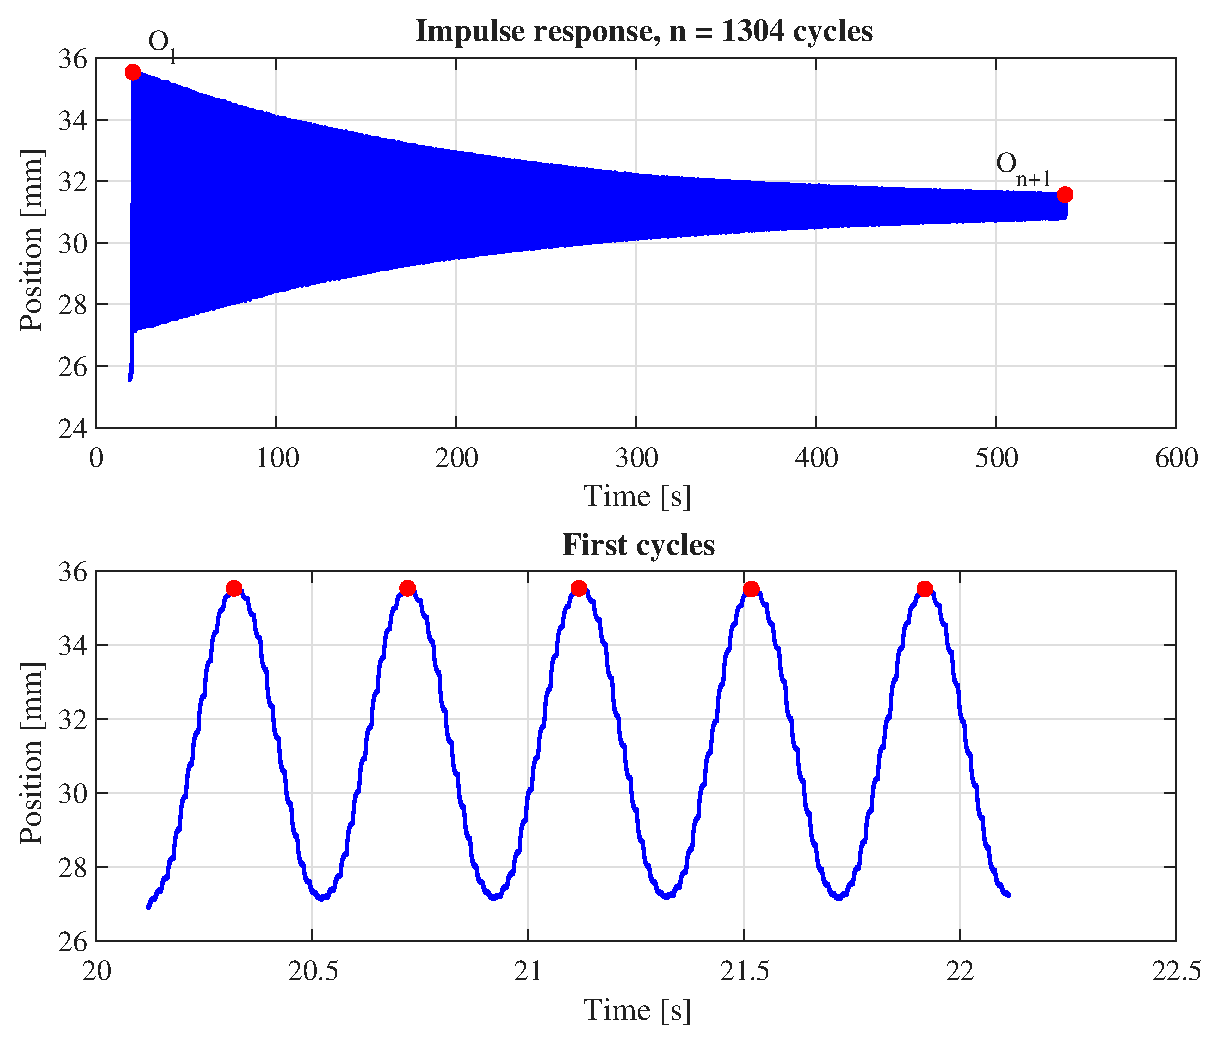
\includegraphics[width=0.85\linewidth]{bs_ringdown.eps}
\caption{Impulse response used to identify $b_s$: the peaks $O_1$ and $O_{n+1}$ of the logarithmic decrement (top) and the first cycles (bottom).}\label{fig:ringdown}
\end{figure}

\subsection{Input Gain and Actuator Time Constant}
\note{An early step test gave 0.66 of the Table 1 gain. Later rig data gave 0.99, i.e.\ Table 1 is right.
Frequency response: sinusoidal inputs plotted on a Bode plot (L2d). The frequency is increased slowly in one run instead of one sine at a time.
Done in closed loop because the actuator integrates. $G = (\text{sine}\to X)/(\text{sine}\to U)$.
The phase at 5--12 Hz favours $\tau_m\approx\SI{18}{ms}$ over the Table 1 value \SI{30.9}{ms}. The measured data are noisy, so the evidence is weak.
$\tau_m = M_eR/(K_fK_b)$; the motor inertia dominates through the fine screw lead.}
\begin{figure}[H]\centering
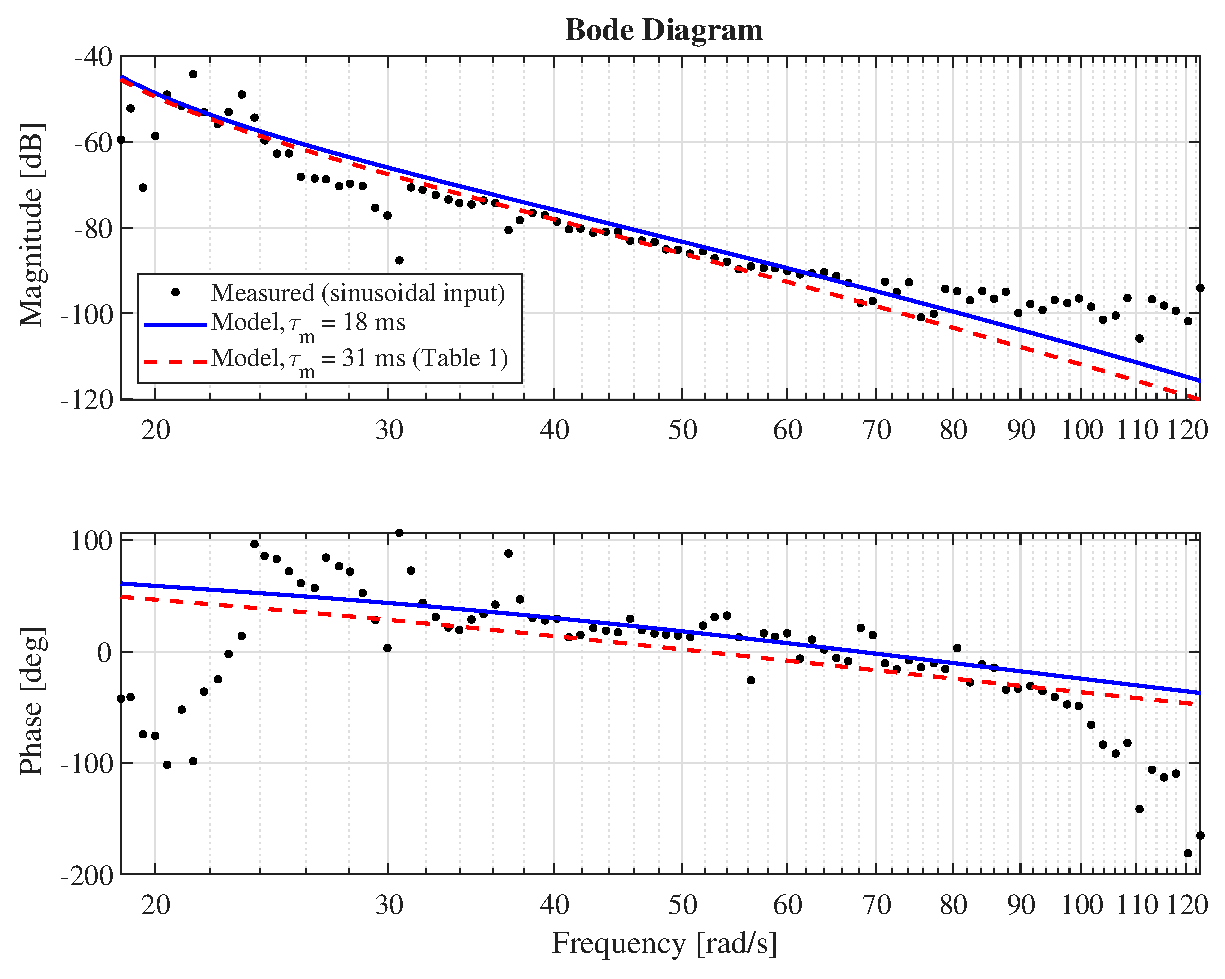
\includegraphics[width=0.8\linewidth]{bode_chirp.eps}
\caption{Measured frequency response (sinusoidal input, run 4) against the model with $\tau_m = \SI{18}{ms}$ and \SI{31}{ms}.}\label{fig:bode}
\end{figure}

\subsection{Model Validation}
% Compare model with measured data (time and/or frequency domain).
\note{Step response against the model. With input gain 0.99 the model predicts the poorly damped 6 Hz oscillation of the first
controller (gain margin 2.2 dB, 5.4--6.5 Hz against 6.0--6.25 Hz on the rig) and the instability of the soft gain set with a few ms of time delay. This is the argument for
trusting the model.}
\begin{figure}[H]\centering
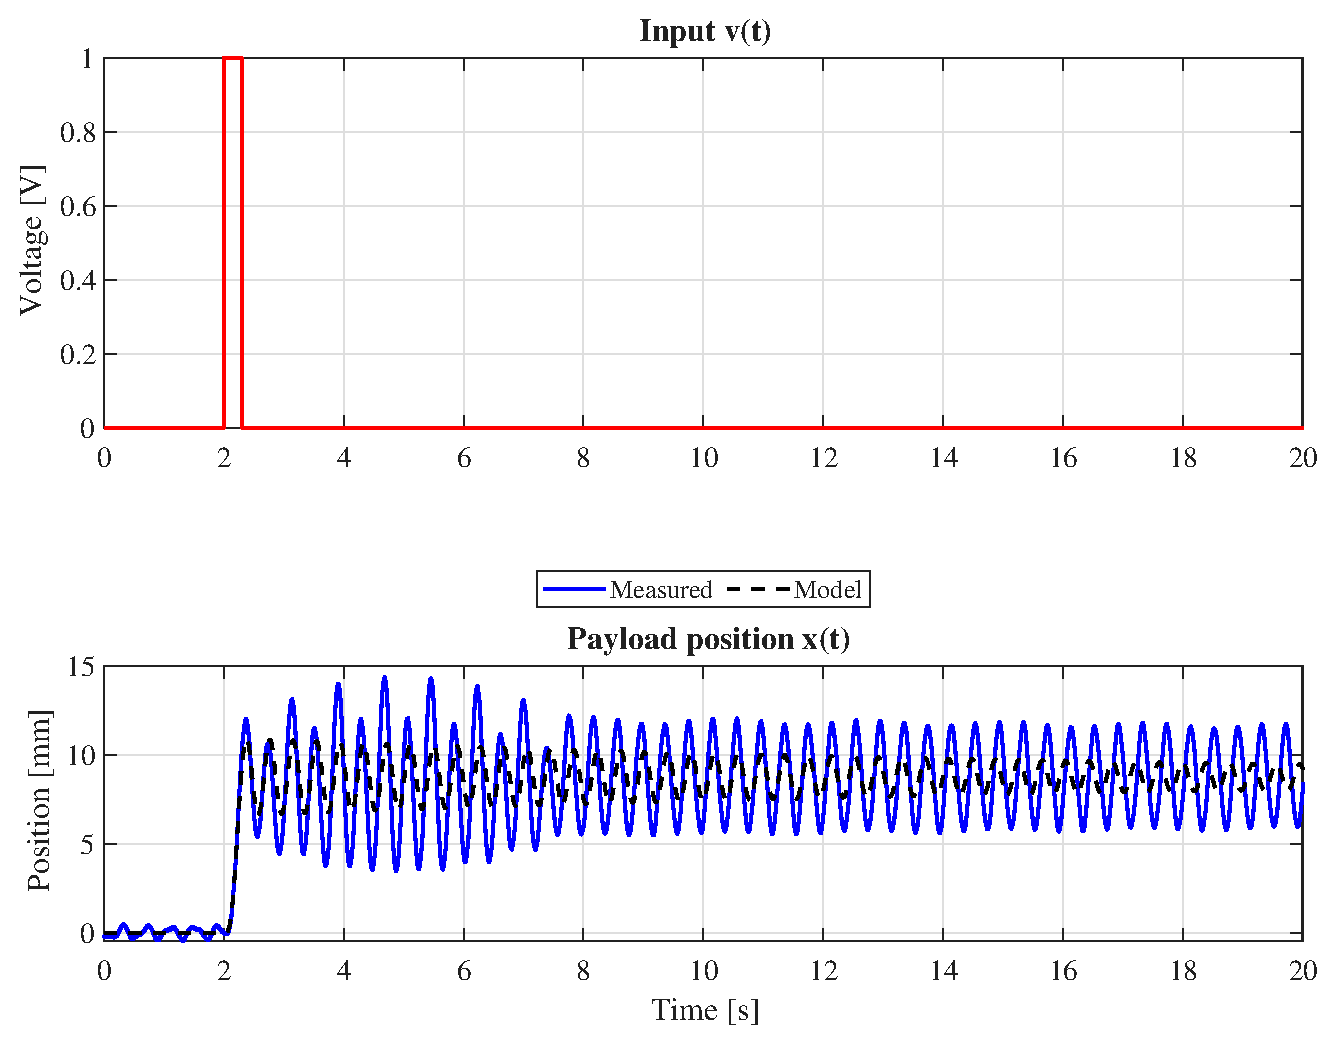
\includegraphics[width=0.8\linewidth]{validate_last_run.eps}
\caption{Open-loop pulse response: rig against model.}\label{fig:validate}
\end{figure}

\subsection{What the Model Does Not Capture}
\note{Unmodelled friction (e.g.\ Coulomb friction) in the ball screw and motor driver: the actuator does not move for small voltages. Treated as uncertainty and handled by integral control (an integrator reduces the steady-state error from friction), not modelled.}
\begin{figure}[H]\centering
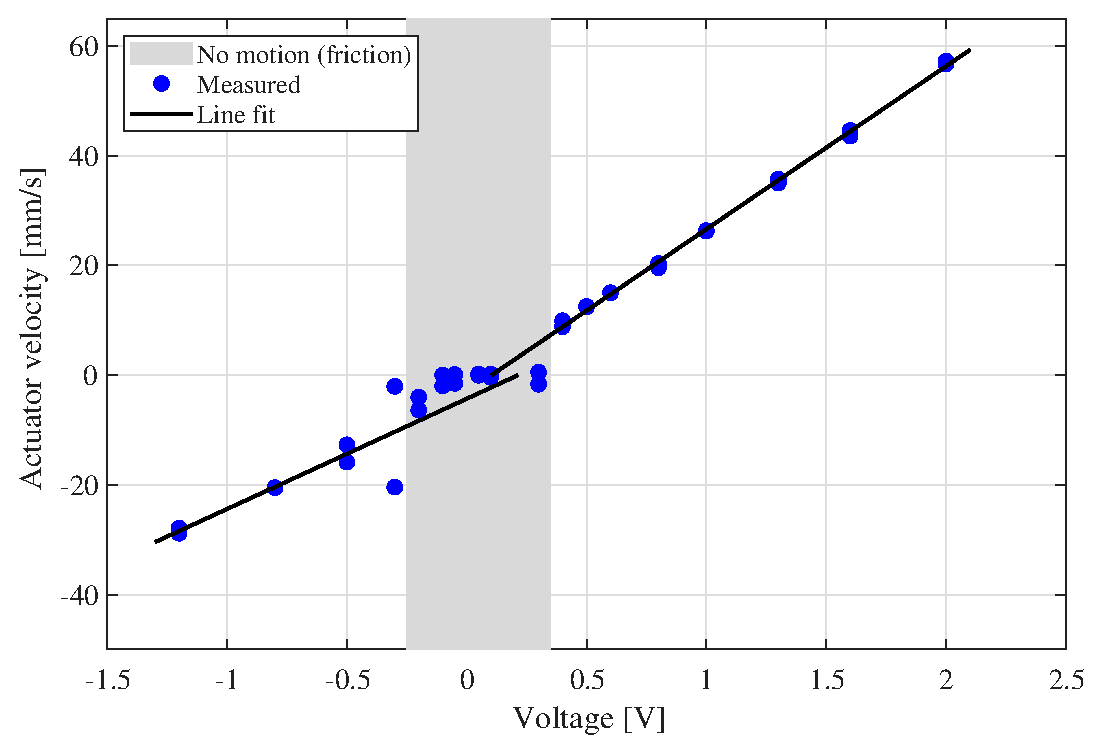
\includegraphics[width=0.75\linewidth]{driver_map.eps}
\caption{Measured motor-driver characteristic: actuator speed against voltage. The actuator does not move for small voltages (friction).}\label{fig:driver}
\end{figure}

\begin{table}[H]\centering
\caption{Parameter uncertainty used for the robustness checks.}
\begin{tabular}{lcc}\toprule
Quantity & Nominal (design) & Range checked\\\midrule
Input gain (relative to Table 1) & 0.99 & 0.66--1.32\\
Actuator time constant $\tau_m$ & \SI{18}{ms} & 12--31\,ms\\
Ball-screw efficiency $\eta$ & 1.0 & 0.66--1.0\\
Payload mass $m_l$ & \SI{0.51}{kg} & 0.36--0.77\,kg\\
Extra time delay & 0 & +5\,ms\\\bottomrule
\end{tabular}\end{table}

%=====================================================================
\section{Controller Design}\label{sec:ctrl}
% Full-state feedback controller and why this design method was chosen.
% How steady-state accuracy is ensured.
\subsection{LQR with Integral Control}
\note{Why LQR and not pole placement: 6--7 states, Bryson's rule gives physical weights, explicit trade-off against voltage \cite{lectures}.
Why integral control and not only a prefilter $N$: the gain estimates ranged 0.66--0.99, $\eta$ is unknown, and a constant voltage is needed to hold the payload.}
The model is augmented with the integral of the tracking error, $\dot x_N = r - C\mathbf{x}$ (with $C\mathbf{x}=x_s$, the measured position):
\begin{equation}
\dot{\mathbf{x}}_a = \begin{bmatrix}A & 0\\ -C & 0\end{bmatrix}\mathbf{x}_a + \begin{bmatrix}B\\0\end{bmatrix} v
+\begin{bmatrix}0\\1\end{bmatrix} r,\qquad
v = -K\hat{\mathbf{x}} + K_e x_N.
\end{equation}
$[K\;\;-K_e]$ minimises $J=\int_0^\infty (\mathbf{x}_a^TQ\mathbf{x}_a + R v^2)\,dt$, with Bryson's rule
$Q_{jj}=1/x_{j,\max}^2$, $R = 1/v_{\max}^2$.

\begin{table}[H]\centering
\caption{Weights from Bryson's rule.}
\begin{tabular}{lcl}\toprule
State & Max.\ value & Reason\\\midrule
$i$ & \SI{5}{A} & motor rated current 5.14\,A\\
$y$ & \SI{25}{mm} & stroke\\
$\dot y$ & \SI{0.15}{m/s} & \\
$x$ & \SI{8}{mm} & \\
$\dot x$ & \SI{20}{mm/s} & \\
$x_s$ & $10^3$ (none) & sensor state, not penalised\\
$x_N$ & \SI{1}{mm\,s} & integral of the error\\
$v$ & \SI{5}{V} & voltage limit\\\bottomrule
\end{tabular}\end{table}

\note{Anti-windup: the integrator is frozen while the voltage is saturated (one line).
Gain-set history: v1 oscillated at 6 Hz on the rig (gain margin 2.2 dB). The v3 selection rule: stable over the whole parameter uncertainty, settling time $t_s\le\SI{2}{s}$, observer poles $\ge2\times$ faster than the controller poles.}

\subsection{Robustness}
\begin{table}[H]\centering
\caption{Robustness of the final gains (v3a). GM = gain margin, PM = phase margin; $\zeta_{\min}$ is the lowest damping ratio of the closed-loop poles.}
\begin{tabular}{lccc}\toprule
Case & GM [dB] & PM [$^\circ$] & $\zeta_{\min}$\\\midrule
Identified plant (gain 0.99, $\tau_m$ 18\,ms, $m_l$ 0.51\,kg) & 7.6 & 39 & 0.52\\
$\tau_m = \SI{31}{ms}$ (Table 1) & 7.8 & -- & 0.25\\
Worst over gain 0.66--1.32, $\tau_m$ 12--31\,ms, $\eta$ 0.66, +5\,ms & -- & -- & 0.17\\
$m_l = \SI{0.66}{kg}$ / \SI{0.77}{kg} & 10.0 / 11.4 & 46 / 49 & 0.53 / 0.43\\
$m_l = \SI{0.36}{kg}$ ($-30\,\%$) & 4.2 & 25 & 0.20\\
$m_l = \SI{0.36}{kg}$, gain 1.32, +5\,ms & 1.7 & 12 & $-0.01$ (unstable)\\\bottomrule
\end{tabular}\end{table}
\note{Discuss the mass rows honestly. A heavier payload increases the margins. A much lighter payload combined with the worst-case gain and
extra time delay is the only case checked where the closed loop goes unstable: a lighter payload raises the spring mode
($f_n\propto 1/\sqrt{m_l}$) towards 6 Hz, where the phase margin is already small.}

%=====================================================================
\section{Observer Design}\label{sec:obs}
% State observer for the unmeasured states and why this method was chosen.
\note{Only $x$ is measured; estimate $i, y, \dot y, \dot x, x_s$. Kalman filter (LQE), because the noise levels are physical or measured:
measurement noise \SI{22}{\micro m}; process noise = voltage uncertainty + 1\,N force disturbance on the payload. Separation principle.
The observer poles are 5.3$\times$ faster than the dominant controller poles. Discretised at $T_s=\SI{0.1}{ms}$.}
\begin{equation}
\dot{\hat{\mathbf{x}}} = A\hat{\mathbf{x}} + Bv + L_{obs}(x_{meas} - C\hat{\mathbf{x}}).
\end{equation}

%=====================================================================
\section{Simulation Results}\label{sec:sim}
% Lift to x0+15 mm, lower to x0+5 mm.
% Lift to x0+20 mm, lower to x0+5 mm (same controller).
% Robustness: uncertain efficiency, model errors, step force / push.
\note{Controller\_test.slx uses the same controller block as the real-time model. Plant: identified model + sensor sampling and lag + measured motor-driver characteristic.
Comment on the figure.}
\begin{figure}[H]\centering
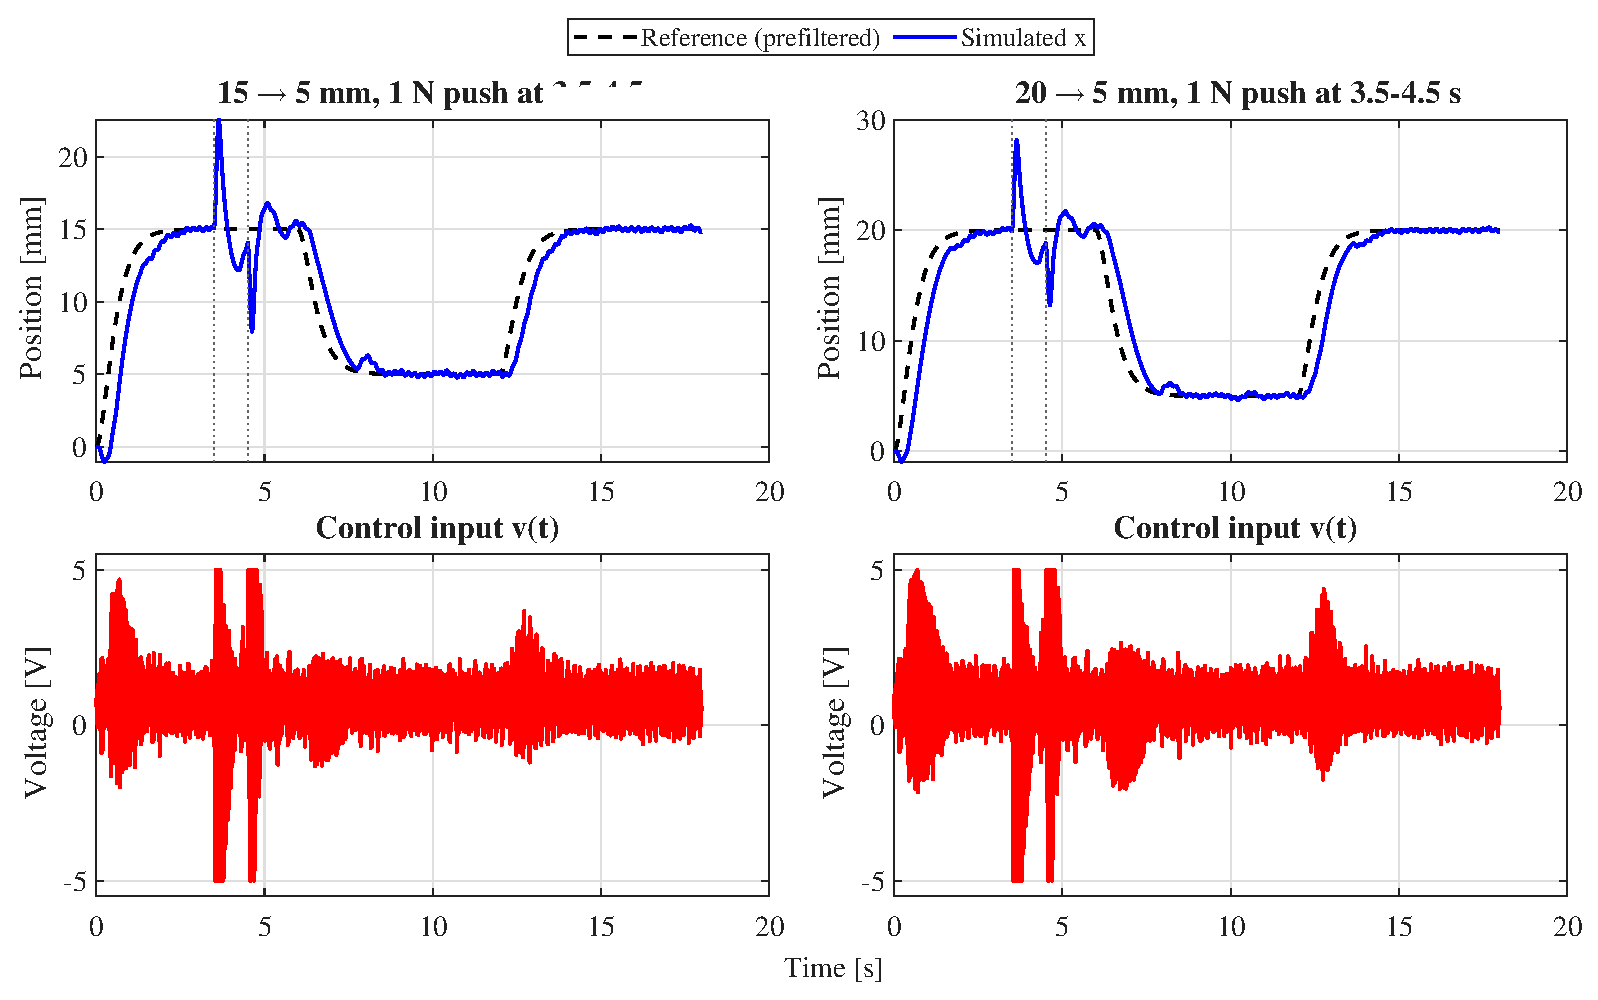
\includegraphics[width=\linewidth]{sim_final.eps}
\caption{Simulation of both reference cases with a 1\,N push (force disturbance) at 3.5--4.5\,s, identified model. The gain range is covered by the robustness table.}\label{fig:simfinal}
\end{figure}

%=====================================================================
\section{Real-Time Implementation}\label{sec:rt}
% Simulink model running on the Speedgoat.
\note{Project\_IOinterface.slx is left untouched; the controller is generated by build\_controller\_model.m. Two additions came from rig testing:
a reference prefilter $1/(0.3s+1)^2$ (outside the loop, so the gain and phase margins don't change; up-step overshoot 20$\to$12\,\%, no saturation at $\pm$5\,V),
and initial conditions at the equilibrium point (observer, integrator and prefilter start at the measured rest position of 1.6\,mm; this removes the large voltage at start-up).}
\begin{figure}[H]\centering
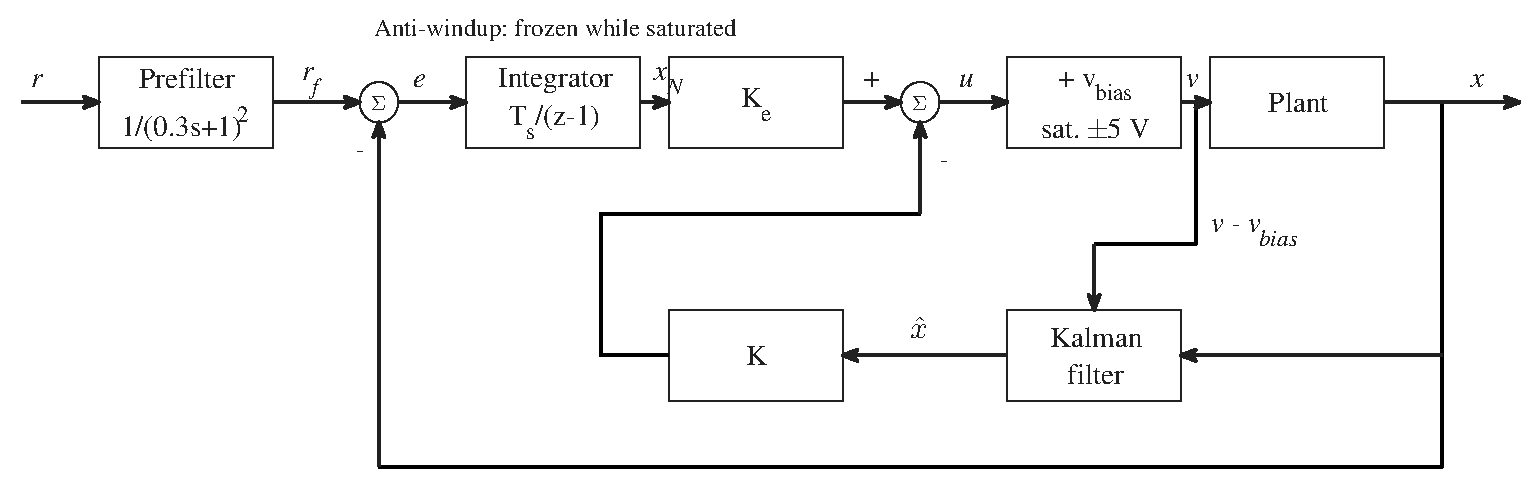
\includegraphics[width=0.9\linewidth]{block_diagram.eps}
\caption{LQG controller structure.}\label{fig:block}
\end{figure}
\begin{figure}[H]\centering
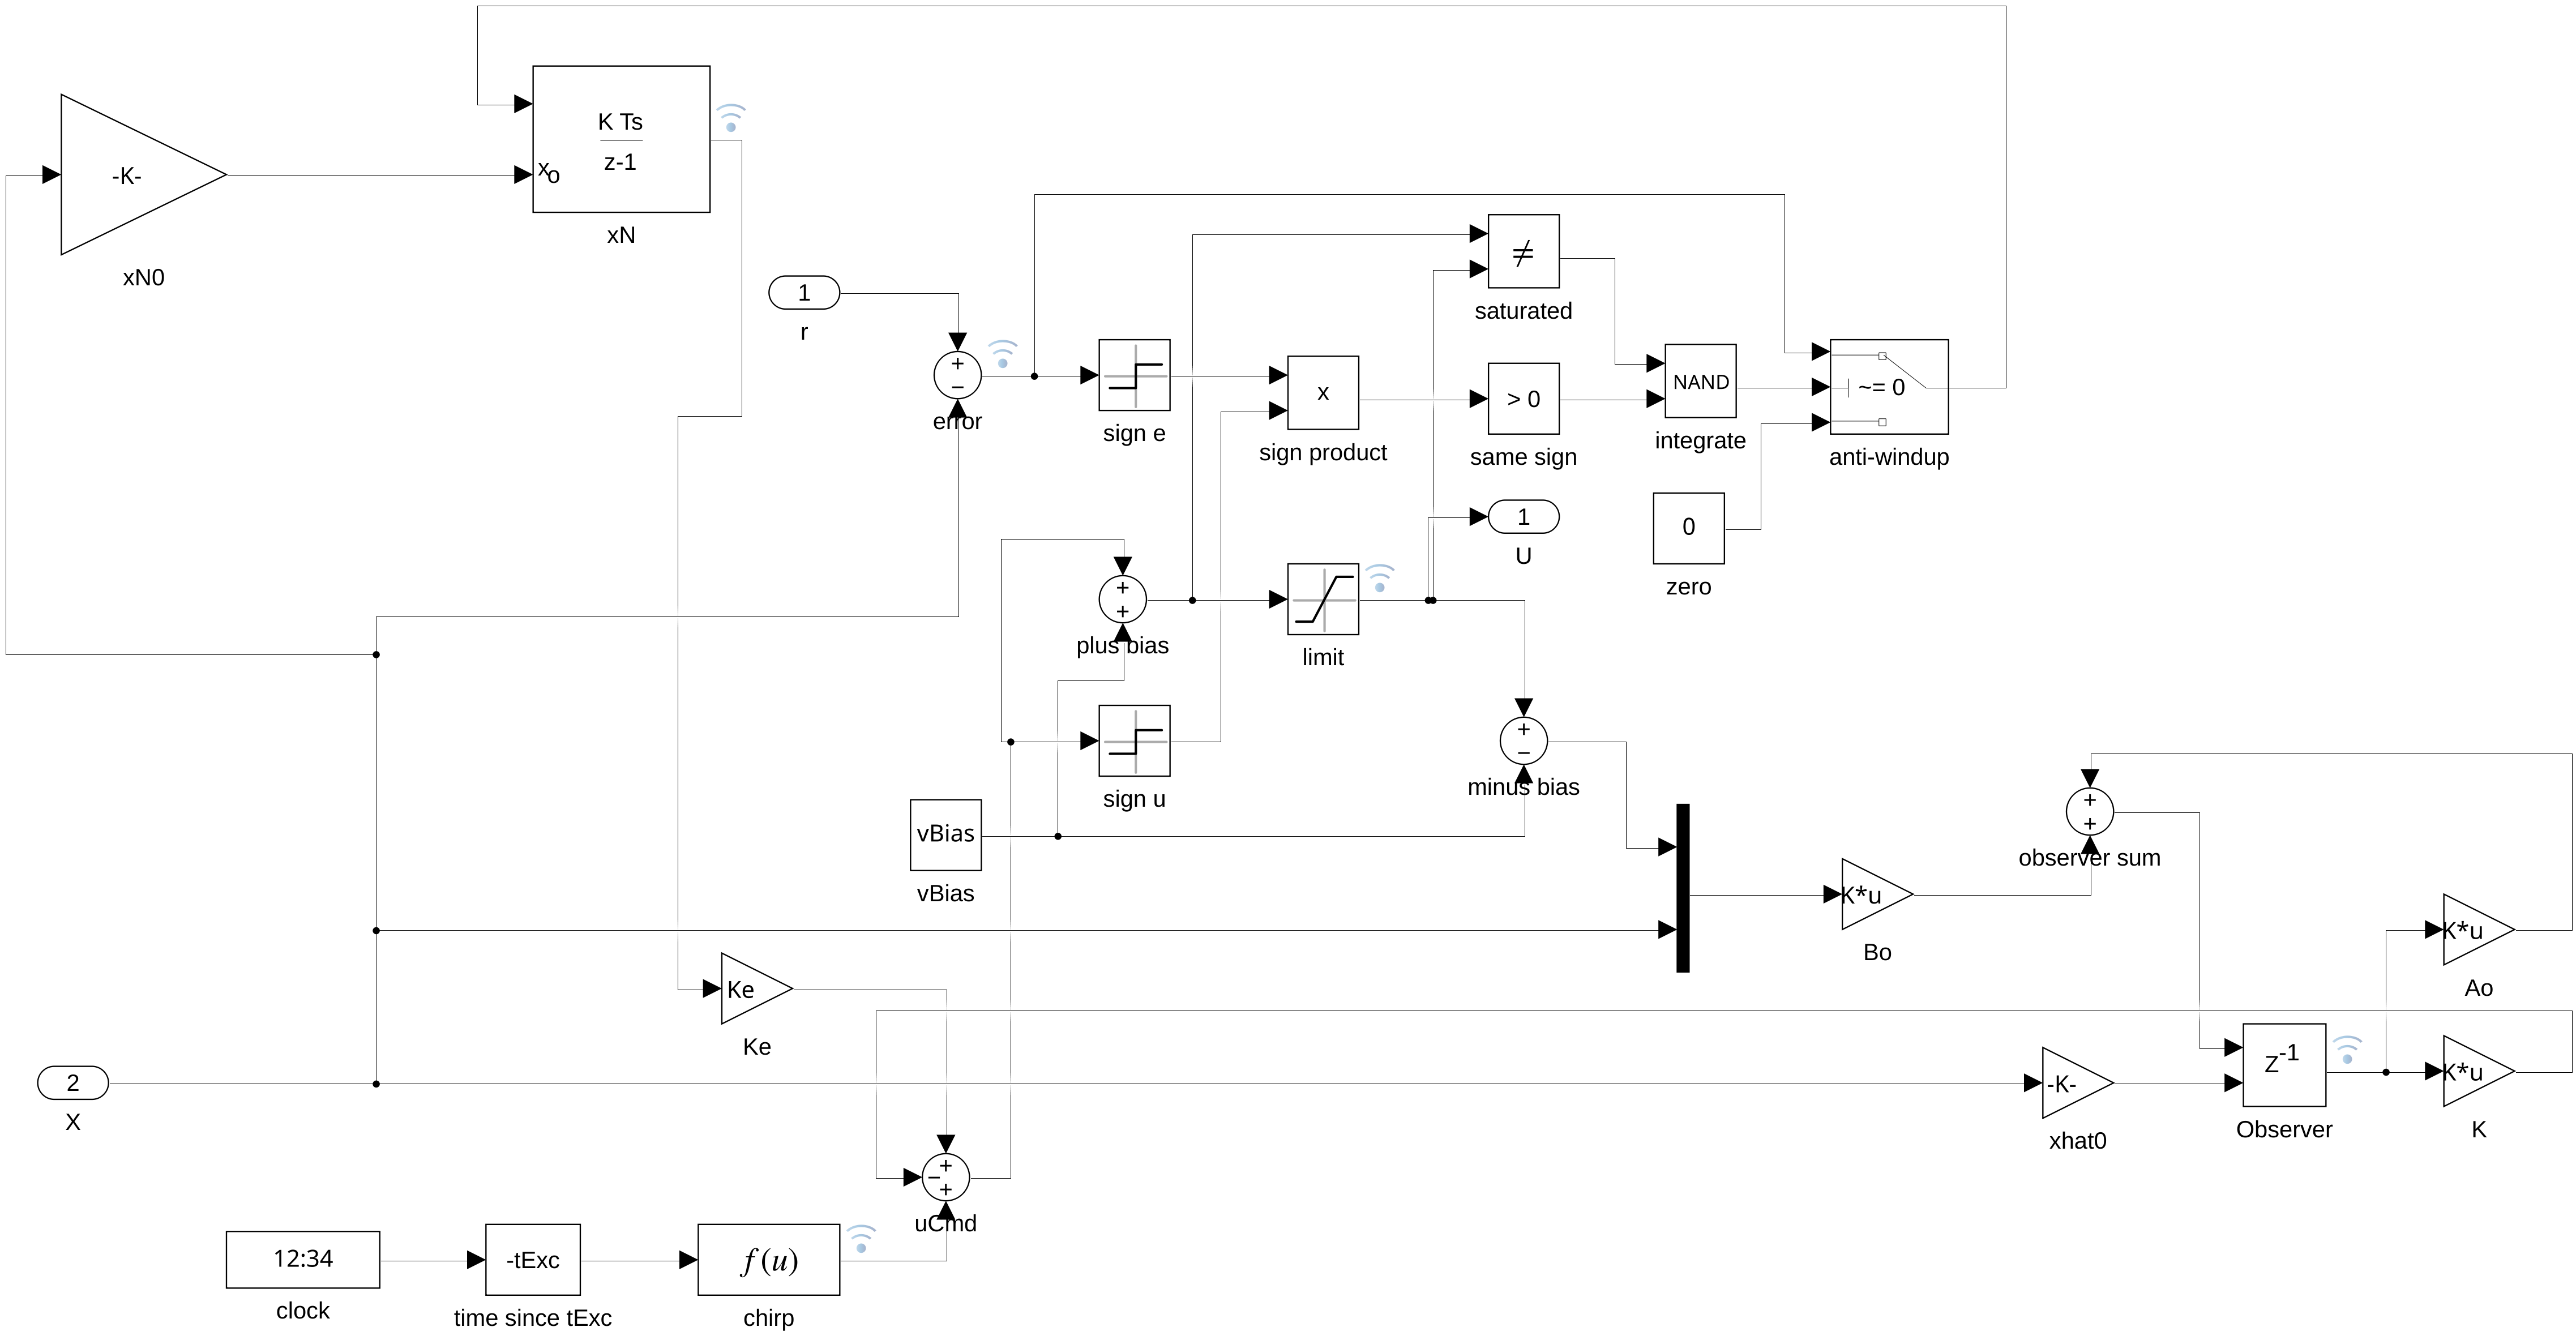
\includegraphics[width=\linewidth]{simulink_controller.png}
\caption{Controller subsystem as implemented in Simulink.}\label{fig:simulink}
\end{figure}

%=====================================================================
\section{Experimental Results}\label{sec:results}
% Same test cases on the real setup. Compare with simulation.
% Reference to the submitted video.
\begin{figure}[H]\centering
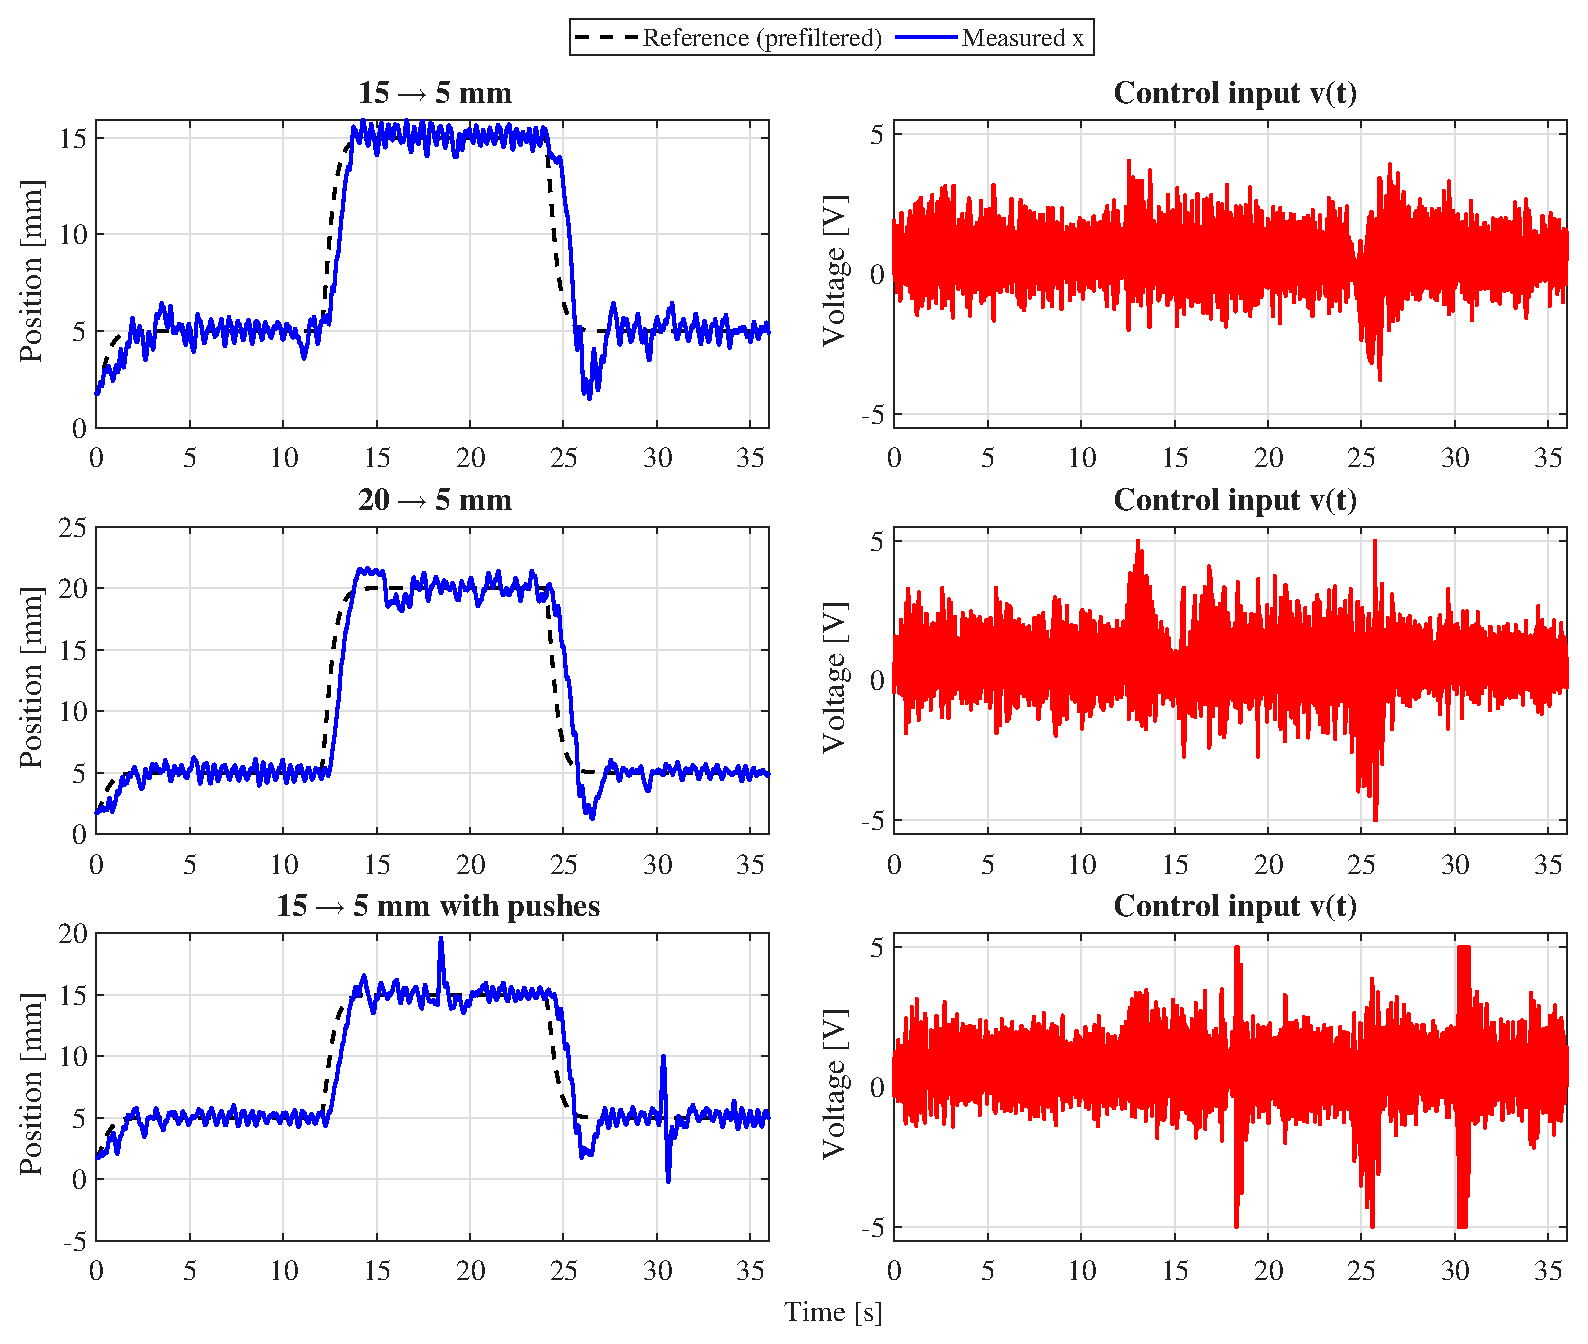
\includegraphics[width=\linewidth]{final_rig_runs.eps}
\caption{Final controller on the rig: 15$\to$5\,mm, 20$\to$5\,mm, and 15$\to$5\,mm with pushes.}\label{fig:rig}
\end{figure}

\begin{table}[H]\centering
\caption{Requirements against rig results.}
\begin{tabular}{p{5cm}p{9cm}}\toprule
Requirement & Result\\\midrule
Steady-state error & Mean error over the last 2\,s of each hold $-0.05$ to $+0.14$\,mm (one dip of $-0.5$\,mm from the friction oscillation)\\
Same controller for both cases & Yes, no retuning\\
$|v|\le\SI{5}{V}$ & At the limit 0--0.5\,\% of the time\\
Stroke 0--25\,mm & Yes (one push release $-0.3$\,mm)\\
Push & Held on reference while pushed; recovers in about 1\,s\\
Overshoot & 11--17\,\% up, 25--33\,\% down\\\bottomrule
\end{tabular}\end{table}

\begin{figure}[H]\centering
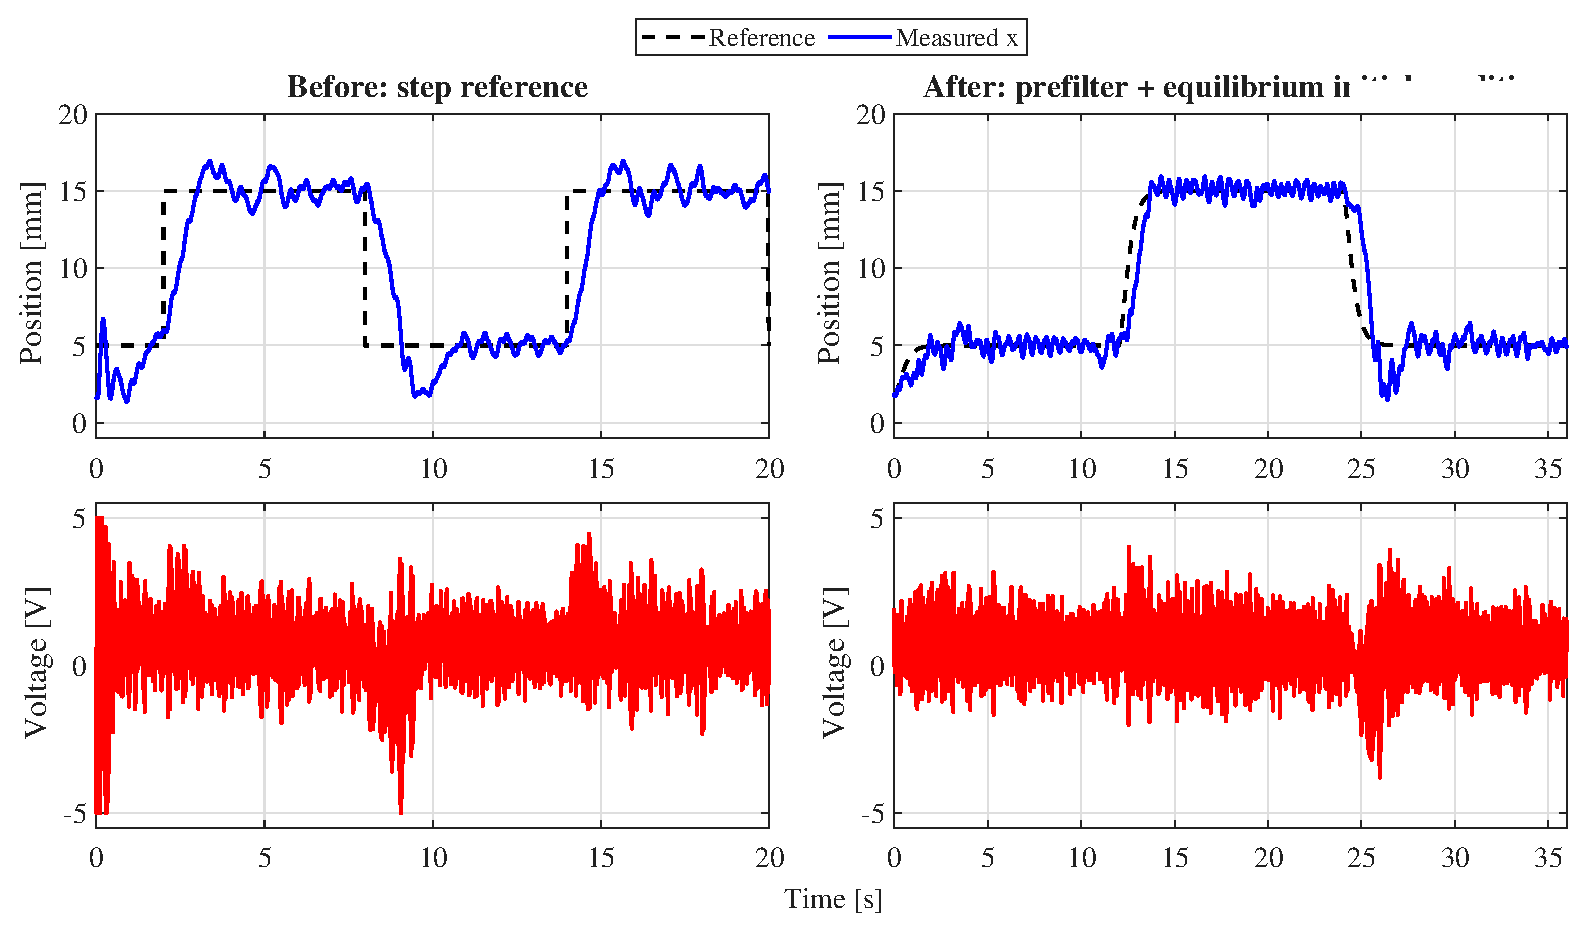
\includegraphics[width=\linewidth]{before_after.eps}
\caption{Rig, 15$\to$5\,mm: first controller with a step reference (left) against the final controller with prefilter and equilibrium initial conditions (right).}\label{fig:beforeafter}
\end{figure}
\note{Push test: release spike $\approx F/k_s$ (1\,N / 132\,N/m $\approx$ 7.6\,mm). This is physics: the integrator has stretched the spring.
Compare with the simulation (the sim underpredicts the down-step overshoot because it does not model friction).
Give the file name of the submitted video here.}

%=====================================================================
\section{Discussion}\label{sec:disc}
\note{The oscillation about the reference and the down-step overshoot come from unmodelled friction in the actuator (it sticks, then jumps). Evidence: the measured driver characteristic (Fig.~\ref{fig:driver}) shows no motion for small voltages, and the oscillation is the same for four different controllers (slower and faster gains), so the controller does not cause it.
What would help: friction compensation, a better driver.}

%=====================================================================
\section{Conclusion}
% What was achieved.
\note{Half a page.}

%=====================================================================
\appendix
\renewcommand{\thesection}{\Alph{section}}
\setcounter{section}{0}
\section{Parameters}
\begin{table}[H]\centering
\begin{tabular}{llll}\toprule
Parameter & Value & Unit & Source\\\midrule
$m_a$ & 0.3 & kg & Table 1\\
$R$ & 0.55 & $\Omega$ & Table 1\\
$L$ & 0.8 & mH & Table 1\\
$k_i$, $k_b$ & 0.036 & Nm/A, V/(rad/s) & Table 1\\
$J_m$ & $72\times10^{-6}$ & kg\,m$^2$ & Table 1\\
$l$ & 0.01 & m & Table 1\\
$\eta$ & 1.0 (model) & -- & Table 1\\
$m_l$ & 0.51 & kg & Table 1\\
$k_s$ & 131.7 & N/m & static test\\
$b_s$ & 0.0048 & Ns/m & impulse response\\
$\tau_m$ & 18 (Table 1: 30.9) & ms & frequency response\\
$\tau_s$ & 10.6 & ms & sensor datasheet + data\\
Holding voltage & 0.6 & V & measured\\\bottomrule
\end{tabular}\end{table}

\section{Controller Gains}
Final gains (v3a), state order $[i,\ y,\ \dot y,\ x,\ \dot x,\ x_s]$, SI units, continuous-time design (discretised in the controller block), $T_s=0.0001$\,s.
\begin{align*}
K &= \begin{bmatrix}\num{0.6493} & \num{3500} & \num{65.49} & \num{-1537} & \num{254} & \num{53}\end{bmatrix},\qquad K_e = 5000,\\
L_{obs} &= \begin{bmatrix}\num{-9.899e+05}\\ \num{5552}\\ \num{2.196e+04}\\ \num{956.7}\\ \num{1.019e+05}\\ \num{340.9}\end{bmatrix}.
\end{align*}


\section{Files and How to Run}
\begin{enumerate}
\item In MATLAB R2025b: \texttt{cd MAS508; setup\_project}
\item \texttt{controller\_design} (gains) $\to$ \texttt{build\_controller\_model} $\to$ \texttt{slbuild('Project\_Controller')}
\item On the target: \texttt{tg = slrealtime; load(tg,'Project\_Controller'); start(tg)}
\item \texttt{report\_figures} regenerates all figures.
\end{enumerate}
